%***************************************************************************************************%
%     File Name: sampleMain.tex
%        Author: Takahiro Yamamoto
% Last Modified: 2016/02/11 13:26:37
%***************************************************************************************************%

\documentclass[10pt, a4paper, onecolumn, oneside]{article}
\title{HasKAL Reference Manual}
\author{Edition 0.1 alpha}
\date{\today}

%----------------------------------------------------------------------------------------------------%
%---------       パッケージ        ------------------------------------------------------------------%
%----------------------------------------------------------------------------------------------------%
\usepackage[top=30mm, bottom=30mm, left=30mm, right=30mm]{geometry}%%マージン
\usepackage{amsmath}%% align
\usepackage[dvipdfmx]{hyperref}%% リンク
\usepackage[dvipdfmx]{graphicx}%% 画像

%---------------------------------------------------------------------------------------------------%
%---------       マクロ        ---------------------------------------------------------------------%
%---------------------------------------------------------------------------------------------------%


%---------------------------------------------------------------------------------------------------%
%---------       ヘッダ        ---------------------------------------------------------------------%
%---------------------------------------------------------------------------------------------------%
\begin{document}
\maketitle
\tableofcontents %目次
\newpage

%----------------------------------------------------------------------------------------------------%
%---------       本文        --------------------------------------------------------------------%
%----------------------------------------------------------------------------------------------------%
\section{Monitor Tools}

\subsection{RayleighMonitor}
\subsubsection{\bf Introduction}
RayleighMonitor is a tool for calculated a quantile value of normalized spectrum of $x(t)$.
The deviation of the calculated quantiles from the expected one in Gaussian noise case
shows deviation of the detector noise from Gaussian distribution.

Normalized spectrogram, $w(t, f)$, of input signal, $x(t)$, is calculated
\begin{align*}
  w(t_i,~f_j) = \frac{ |~{\rm STFT}[x(t)]~| }{S_{\rm 0}(f)},
\end{align*}
where $1\leq i\leq N$, ~$1\leq j\leq M$ and $S_{\rm 0}(f)$ is a normalization factor.
Normalization factor can be estimated
\begin{align*}
  S_{\rm 0}(f) = |~{\rm FFT}[x(t)]~|.
\end{align*}
P-quantile value of input signal is calculated from normalized spectrogram as the function of time and frequency,
$Q(P;~f_l)$ where $1\leq l\leq M/m$, $m(l-1)-1\leq j\leq ml$
and $m = {\rm d}f/{\rm d}f_{\rm fft} = {\rm d}f~{\rm d}t_{\rm fft}$

\subsubsection{{\bf Function:} rayleighMonWaveData}
{\tt ~ rayleighMonWaveData p secfft df x0 xt\\}

This function compute p-quantile value, $Q(p;~f)$, of the input signal, $x(t)$, as the function of frequency, $f$.
The arguments are:
\begin{itemize}
\item {\tt p}: Input. The list of dimensionless p-values ($0 \leq p \leq 1$).
\item {\tt secfft}: Input. The data length for short time Fourier transform in seconds.
\item {\tt df}: Input. The frequency resolution of $Q(p;~f)$ in Hertz
\item {\tt x0}: Input. The time series signal for estimating averaged spectrum
\item {\tt xt}: Input. The time series for calculating quantile value $Q(p;~f)$
\item {\tt q}: Output. The quantile value of input signal $Q(p;~f)$.
\end{itemize}

\subsubsection{{\bf Example:} rayleighMon}
This program calculates the $Q(p;~f)$ of the input signal.\\

{\noindent \bf Typical usage:} {\tt rayleighMon param.conf file.lst}
{\footnotesize
\begin{verbatim}
  import Data.Maybe (catMaybes)
  import System.Environment (getArgs)

  import HasKAL.DetectorUtils.Detector (Detector(..))
  import HasKAL.FrameUtils.Function (readFrameWaveData')
  import HasKAL.Misc.ConfFile (readFileList, readConfFile)
  import HasKAL.MonitorUtils.RayleighMon.RayleighMon (rayleighMonWaveData)
  import HasKAL.PlotUtils.HROOT.PlotGraph
  import HasKAL.WaveUtils.Data (WaveData(..))
  import HasKAL.WaveUtils.Function (catWaveData)

  main = do
    {-- arg check --}
    args <- getArgs
    (conf, lst) <- case length args of
                    2 -> return (args!!0, args!!1)
                    _ -> error Usage: rayleighMon conffile filelist"

    {-- read param --}
    filelist <- readFileList lst
    ([ch, dtfft, df], [qs]) <- readConfFile conf ["channel", "dtfft", "df"] ["quantile"]

    {-- read data --}
    mbWd <- mapM (readFrameWaveData' KAGRA ch) filelist
    let wd = case catMaybes mbWd of
              [] -> error "Can't find file."
              xs -> catWaveData xs

    {-- main --}
    let result = rayleighMonWaveData (map read qs) (read dtfft) (read df) wd wd
        lineType = concat $ replicate (length qs) [LinePoint, Line]
        colors = concatMap (replicate 2) [RED, BLUE, PINK, GREEN, CYAN, YELLOW, BLACK]
        title = ch ++ ": " ++ (show . fst . startGPSTime $ wd) ++ " ~ " ++ (show . fst . stopGPSTime $ wd)
    oPlotV Linear lineType 1 colors ("frequency [Hz]", "normalized noise Lv.") 0.05
    title "X11" ((0,0),(0,0)) $ concatMap (\(x,y) -> [x,y]) result

\end{verbatim}
}


{\noindent \bf Param file format:} {\tt param.conf}
{\footnotesize
\begin{verbatim}
  channel: X1:HOGE-XX  # channel name
  quantile: 0.5 0.95   # list of dimensionless p-value
  dtfft: 1             # data length for STFT in seconds
  df: 16               # frequency resolution of Q(p;~f) in Hertz

\end{verbatim}
}

{\noindent \bf List file format:} {\tt file.lst}
{\footnotesize
\begin{verbatim}
  /path/to/framefile/a.gwf
  /path/to/framefile/b.gwf

\end{verbatim}
}

\begin{figure}[t]
 \begin{center}
    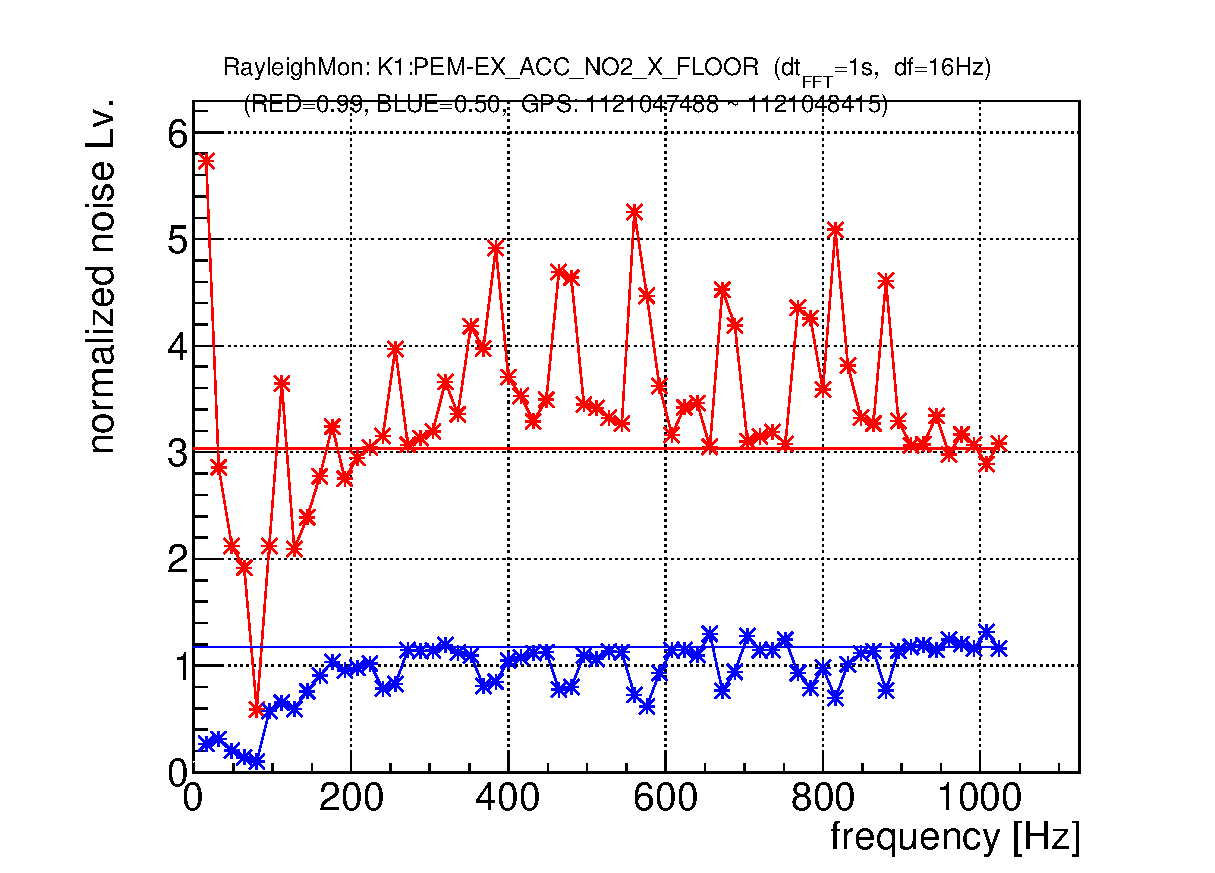
\includegraphics[width=0.9\hsize]{fig/RayleighMon/sample1.eps}
    \caption{sample plot of rayleighMonitor}
 \end{center}
\end{figure}

{\noindent \small contact person: Takahiro Yamamoto (\tt yamamoto@yukimura.hep.osaka-cu.ac.jp)}


\newpage

\subsection{StudentRayleighMonitor}
\subsubsection{\bf Introduction}
StudentRayleighMonitor is a tool for investigating stationarity non-Gaussianity of input signal $x(t)$
by assuming detector noise distributed the Student-t distribution.
In this assumption, non-Gaussianity is represented by only one parameter, $\nu$, which shows weight of tail of the distribution.
Non-Gaussianity, $\nu$, is computed as the function of time, $t$, and frequency, $f$, from normalized spectrum of $x(t)$.

Normalized spectrogram, $w(t, f)$, of input signal, $x(t)$, is calculated
\begin{align*}
  w(t_i,~f_j) = \frac{ |~{\rm STFT}[x(t)]~| }{S_{\rm 0}(f)},
\end{align*}
where $1\leq i\leq N$, ~$1\leq j\leq M$ and $S_{\rm 0}(f)$ is a normalization factor.
Normalization factor can be estimated
\begin{align*}
  S_{\rm 0}(f) = |~{\rm FFT}[x(t)]~|.
\end{align*}
P-quantile value of input signal is calculated from normalized spectrogram as the function of time and frequency,
$Q_{P}(t_k, f_l)$ where $1\leq k\leq N/n$, $1\leq l\leq M/m$, $n(k-1)+1\leq i\leq nk$ ,
$m(l-1)-1\leq j\leq ml$, $n = {\rm d}t/{\rm d}t_{\rm fft}$ and $m = {\rm d}f/{\rm d}f_{\rm fft} = {\rm d}f~{\rm d}t_{\rm fft}$

On the other hand, theoretical quantile value in the Student-t noise case can be described
\begin{align*}
  Q_{\rm sr}(\sigma,\nu;P) = \sigma\sqrt{\frac{\nu(1-(1-P)^{2/\nu})}{(1-P)^{2/\nu}}}
\end{align*}

Degree of non-Gaussianity $\nu$ is calculated from P-quantile value of data and theoretical quantile value.
\begin{align*}
  \nu(t_k, f_l) = \mathop{\rm arg~min}\limits_{\nu} | Q_{P=P_0}(t_k,f_l) - Q_{\rm sr}(\sigma,\nu;P=P_0)|
\end{align*}

\subsubsection{{\bf Function:} studentRayleighMonWaveData}
{\tt studentRayleighMonWaveData p secfft chunck dt df x0 xt\\}

This function compute the non-Gaussianity, $\nu$, of the input signal, $x(t)$, as the function of time, $t$, and frequency, $f$.
The arguments are:
\begin{itemize}
\item {\tt p}: Input. The dimensionless p-value ($0 \leq p \leq 1$).
\item {\tt secfft}: Input. The data length for short time Fourier transform in seconds.
\item {\tt chunck}: Input. The data length for estimating $\nu(f)$ in seconds. ({\tt secfft} $\leq$ {\tt chunck})
\item {\tt dt}: Input. The time resolution of $\nu(t,~f)$ in seconds.
\item {\tt df}: Input. The frequency resolution of $\nu(t, f)$ in Hertz
\item {\tt x0}: Input. The time series signal for estimating averaged spectrum
\item {\tt xt}: Input. The time series for estimating $\nu(t,~f)$
\item {\tt nu}: Output. The dimensionless non-Gaussian parameter $\nu(t,~f)$.
\end{itemize}

\subsubsection{{\bf Example:} studentRayleighMon}
This program calculates the $\nu(t, f)$ of the input signals.\\

{\noindent \bf Typical usage:} {\tt studentRayleighMon param.conf file.lst}
{\footnotesize
\begin{verbatim}
  import Data.Maybe (catMaybes)
  import System.Environment (getArgs)

  import HasKAL.DetectorUtils.Detector (Detector(..))
  import HasKAL.FrameUtils.Function (readFrameWaveData')
  import HasKAL.Misc.ConfFile (readFileList, readConfFile)
  import HasKAL.MonitorUtils.SRMon.StudentRayleighMon (studentRayleighMonWaveData)
  import HasKAL.PlotUtils.HROOT.PlotGraph3D
  import HasKAL.WaveUtils.Data (WaveData(..))
  import HasKAL.WaveUtils.Function (catWaveData)

  main = do
    {-- arg check --}
    args <- getArgs
    (conf, lst) <- case length args of
                    2 -> return (args!!0, args!!1)
                    _ -> error "Usage: rayleighMon conffile filelist"

    {-- read param --}
    filelist <- readFileList lst                                                                                    
    ([ch, q, dtfft, dt, lap, df], _) <- readConfFile conf ["channel", "quantile", "dtfft"
                                                          , "dt", "overlap", ``df"] []

    {-- read data --}
    mbWd <- mapM (readFrameWaveData' KAGRA ch) filelist
    let wd = case catMaybes mbWd of
              [] -> error "Can't find data"
              xs -> catWaveData xs

    {-- main --}
    let result = studentRayleighMonWaveData (read q) (read dtfft)
                    (read dt) (read dt - read lap) (read df) wd wd
        title = ch ++ ": " ++ (show . fst . startGPSTime $ wd)
                   ++ " ~ " ++ (show . fst . stopGPSTime $ wd)
    histgram2dM Linear COLZ ("time [s]", "frequency [Hz]", "nu")
       title "X11" ((0,0),(0,0)) $ result

\end{verbatim}
}

{\noindent \bf Param file format:} {\tt param.conf}
{\footnotesize
\begin{verbatim}
  channel: X1:HOGE-XX  # channel name
  quantile: 0.95       # dimensionless p-value
  dtfft: 1             # data length for STFT in seconds
  dt: 128              # time resolution of \nu(t,f) in seconds
  overlap: 124         # data overlap in seconds
  df: 16               # frequency resolution of \nu(t,f) in Hertz

\end{verbatim}
}

{\noindent \bf List file format:} {\tt file.lst}
{\footnotesize
\begin{verbatim}
  /path/to/framefile/a.gwf
  /path/to/framefile/b.gwf

\end{verbatim}
}

\begin{figure}[t]
  \begin{center}
    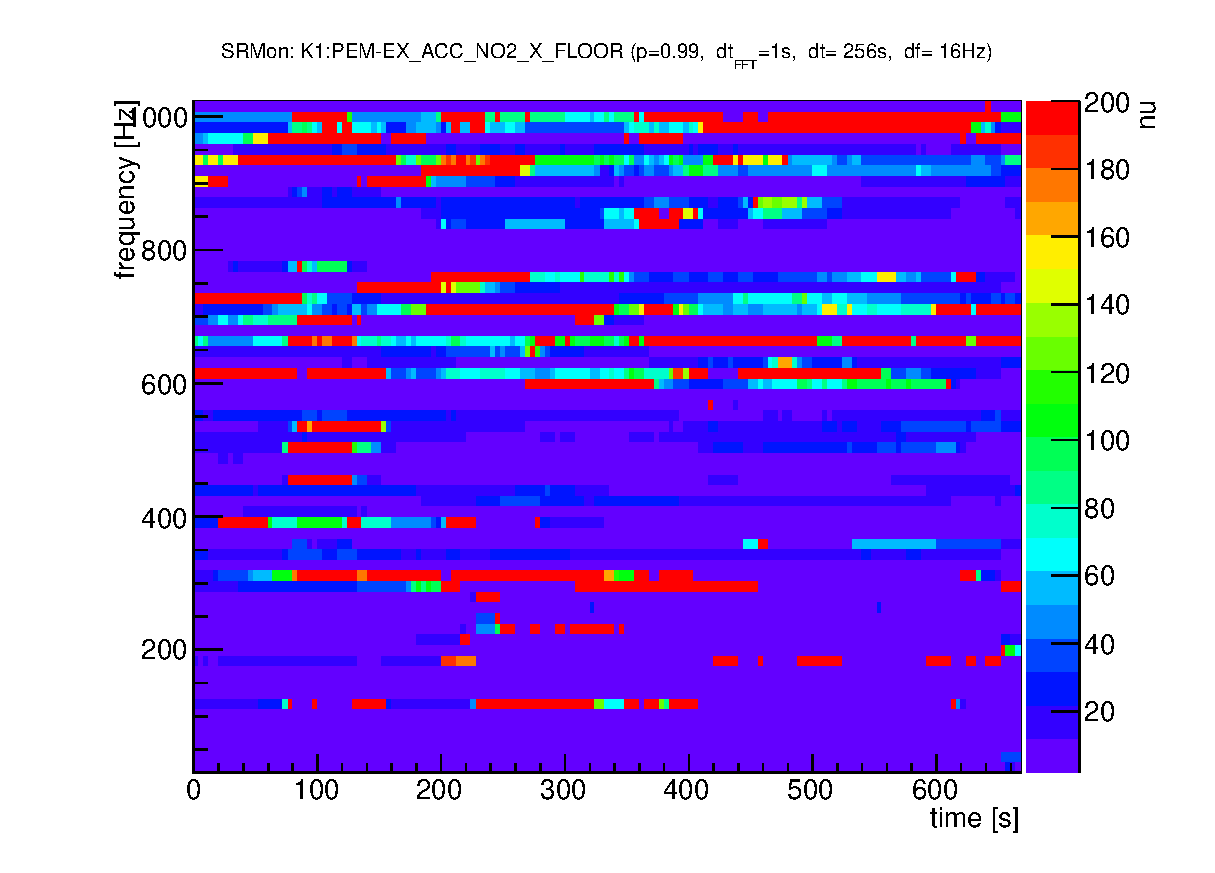
\includegraphics[width=0.9\hsize]{fig/StudentRayleighMon/sample1.eps}
    \caption{sample plot of studentRayleighMonitor}
  \end{center}
\end{figure}

{\noindent \small contact person: Takahiro Yamamoto (\tt yamamoto@yukimura.hep.osaka-cu.ac.jp)}


\newpage

\subsection{RMSMonitor}
\subsubsection{\bf Introduction}
The RMSMonitor is a tool to investigate the non-stationary behavior of the input time series $x(t)$ by calculating the band-limited root-mean square(for short RMS) values.

The RMS values, $\rho_{RMS}(t)$, of input time series, $x(t)$, are calculated as 
\begin{align}
	\rho_{RMS}(t) = \sqrt{ \int_{f_1}^{f_2} |\tilde{x}(f)|^2 df } \label{RMS}
\end{align}
where $f_1$ and $f_2$ are the frequency band and $\tilde{x}(f)$ is the input frequency domain signal calculated by FFT as,
\begin{align*}
  \tilde{x}(f) = {\rm FFT}[x(t)].
\end{align*}


\subsubsection{{\bf Function:} rmsMon}
{\tt rmsMon nmon fs ys freq\\}

This function compute the RMS, $\rho_{RMS}(t)$, of the input time series $x(t)$.
The time series $x(t)$ are divided into small chunks. The RMS value is calculated from each chunk. The number of chunks are calculated by $ N_{ys} / {\tt nmon}$, where $N_{ys}$ is the number of samples of input time series.\\
The arguments are:
\begin{itemize}
\item {\tt nmon}: [Input] The number of samples in one chunk.
\item {\tt fs}: [Input] The sampling frequency of input time series.
\item {\tt ys}: [Input] The input time series.
\item {\tt freq}: [Input] The frequency bands [$f_1:f_2$] described in Eq. (\ref{RMS}). 
\item {\tt {RMS}}: [Output] The calculated RMS values. 
\end{itemize}


\subsubsection{{\bf Function:} rmsMonWaveData}
{\tt rmsMonWaveData nmon freq wd\\}

This function compute the RMS, $\rho_{RMS}(t)$, of the input time series $x(t)$.
The difference between {\tt rmsMon} and {\tt rmsMonWaveData} is the type of input time series.
{\tt rmsMonWaveData} uses WaveData type instead of the time series $x(t)$.
The other arguments are same as {\tt rmsMon}.\\
The arguments are:
\begin{itemize}
\item {\tt nmon}: [Input] The number of samples in one chunk.
\item {\tt wd}: [Input] The input data ({\tt WaveData} type).
\item {\tt freq}: [Input] The frequency bands [$f_1:f_2$] described in Eq. (\ref{RMS}). 
\item {\tt {RMS}}: [Output] The calculated RMS values. 
\end{itemize}


\subsubsection{{\bf Example:} studentRayleighMon}
This program calculates the $\rho_{RMS}$ of the input time series.
Examples of RMSMon are described in Fig. \ref{fig:RMS1} and \ref{fig:RMS2}.


\begin{figure}[ht]
  \begin{center}
    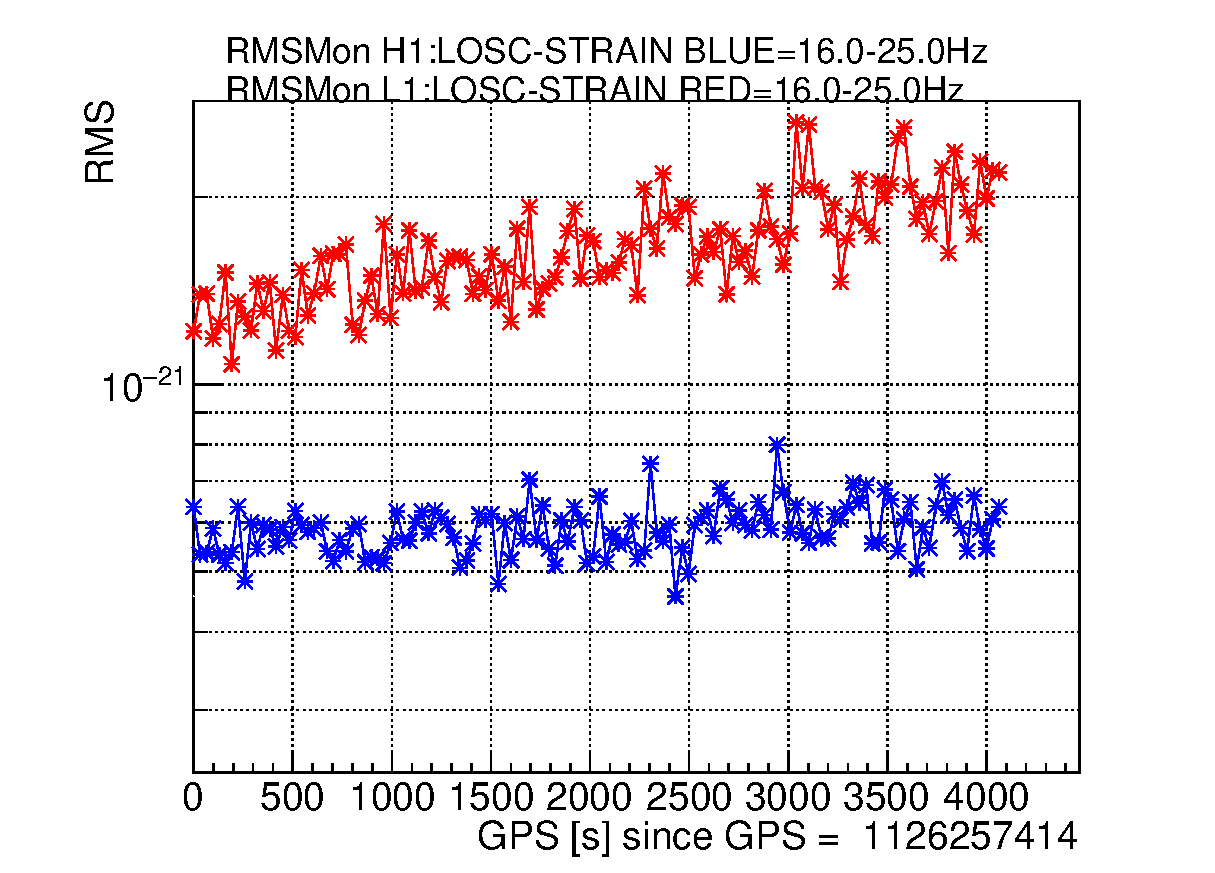
\includegraphics[width=0.9\hsize]{./fig/RMSMon/sample_16-25.eps}
    \caption{Sample plot of RMSMon. The duration of one chunk is 32s. The frequency bands is [16:25]Hz}
     \label{fig:RMS1}
  \end{center}
\end{figure}

\begin{figure}[t]
  \begin{center}
    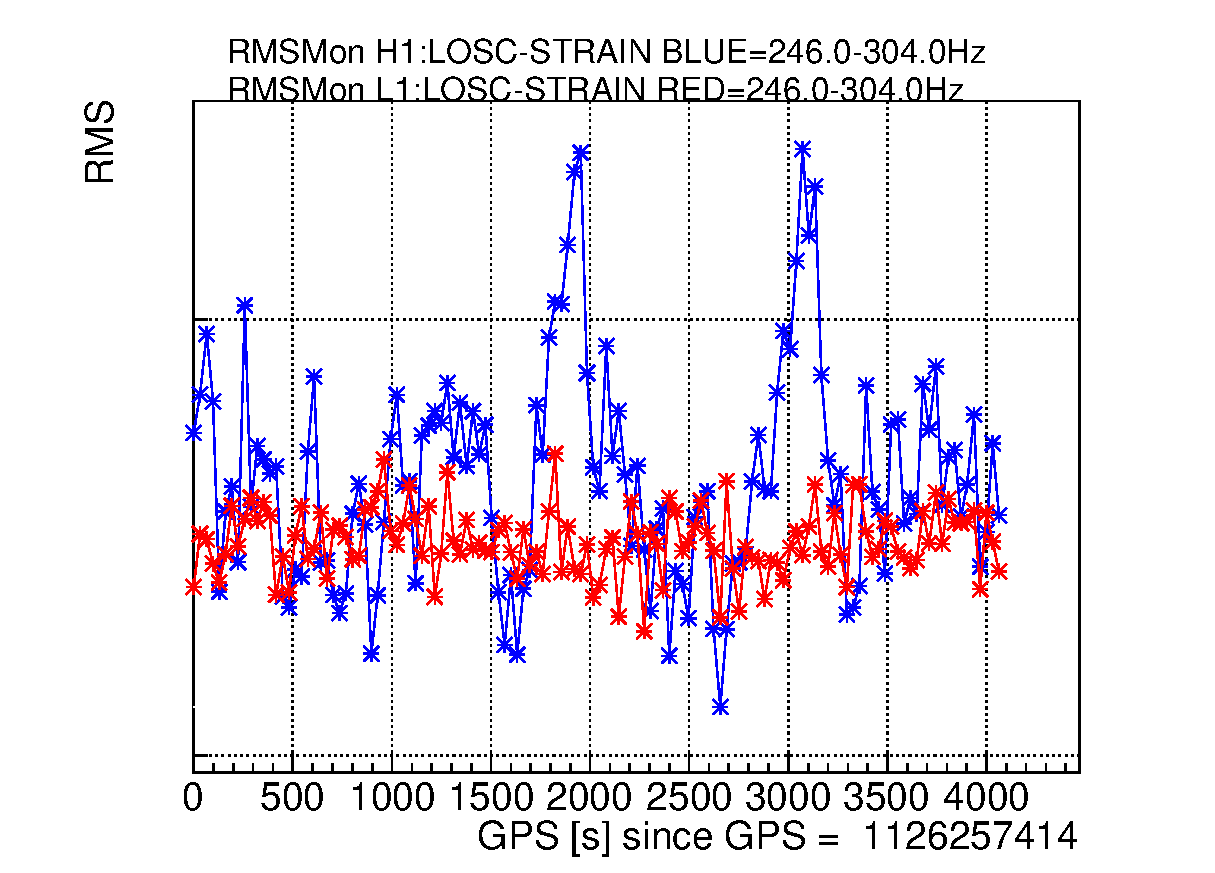
\includegraphics[width=0.9\hsize]{./fig/RMSMon/sample_246-304.eps}
    \caption{Sample plot of RMSMon. The duration of one chunk is 32s. The frequency bands is [246:304]Hz}
     \label{fig:RMS2}
  \end{center}
\end{figure}

{\noindent \small contact person: Hirotaka Yuzurihara (\tt yuzurihara@yukimura.hep.osaka-cu.ac.jp)}


\newpage

\subsection{LineTrackingMonitor}
\newpage
\subsubsection{\bf Introduction}
LineTrackingMonitor is a tool to monitor various lines included in the strain data.
The amplitude and frequency are tracked.


\subsubsection{{\bf Function:} butterBandPass}
{\tt ~ butterBandPass dat fs flow fhigh order\\}
This applies a Butterworth bandpass filter of given cutoff frequencies and filter order to given data.

The arguments are:
\begin{itemize}
\item {\tt dat}: Input. data
\item {\tt fs}: Input. Sampling frequency [Hz]
\item {\tt flow}: Input. Lower cutoff frequency [Hz]
\item {\tt fhigh}: Input. Higher cutoff frequency [Hz]
\item {\tt order}: Input. Filter order
\end{itemize}

It should be noted that this filter is a zero-phase filter (so called filtfilt), so the effective filter order is twice your input value (For example, if you set order $= 5$, the actual filter order becomes ten).


\subsubsection{{\bf Function:} nha}
{\tt ~ nha dat fs nsig nframe nshift nstart nend tlength\\}


The arguments are:
\begin{itemize}
\item {\tt dat}: Input.
\item {\tt fs}: Input. Sampling frequency [Hz]
\item {\tt nsig}: Input. The number of signals (lines) to extract
\item {\tt nframe}: Input. Frame length
\item {\tt nshift}: Input. Shift length
\item {\tt nstart}: Input. The start point
\item {\tt nend}: Input. The end point
\item {\tt tlength}: Input. Time length of data
\end{itemize}


\subsubsection{Sample plots of LineTrackingMonitor}

\begin{figure}[t]
 \begin{center}
    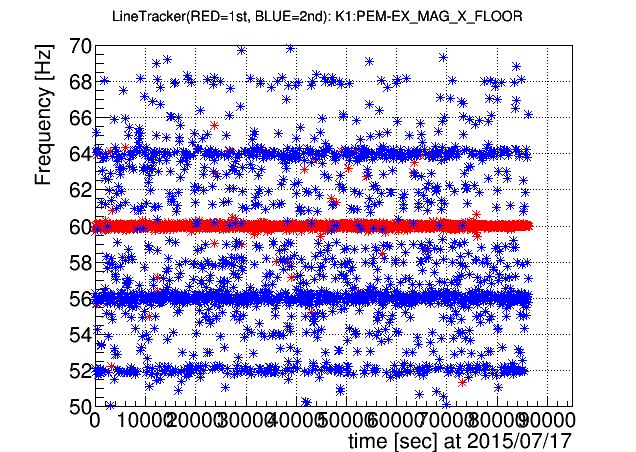
\includegraphics[width=0.9\hsize]{fig/LineTrackingMon/sample_freq.png}
    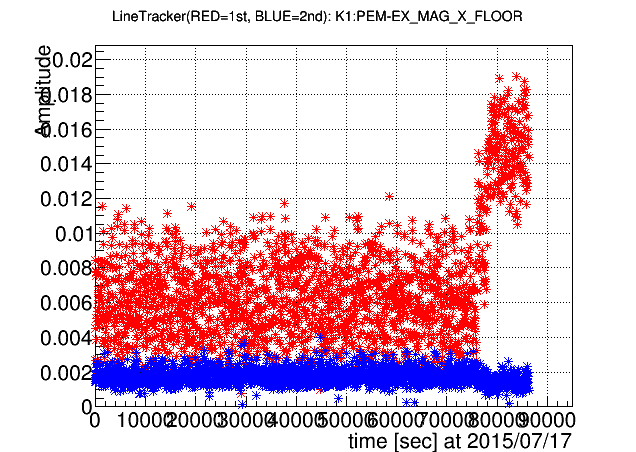
\includegraphics[width=0.9\hsize]{fig/LineTrackingMon/sample_amp.png}
    \caption{sample plots of frequency (top) and amplitude (bottom) of LineTrackingMonitor}
 \end{center}
\end{figure}

{\noindent \small contact person: Koh Ueno (\tt ueno@gwv.hep.osaka-cu.ac.jp)}


\newpage


\end{document}
